Before talking about the electronic system that is used for reading SiPM, we have to keep in mind that we are using SiPM arrays in TRITIUM detector. The electronic system used to process and analyze these output signals is PETSYS \cite{PETSYS}, which is a commercial system prepared to work with SiPM matrices from Hamamatsu, which is the SiPM company chosen for us.

Petsys system, Figure \ref{fig:PETSYS}, is a complete acquisition and digitization system that is capable of working with up to 1024 SiPM arranged in matrices of up to 64 SiPM per matrix. This capacity is necessary because, as we will see in chapter \ref{chap:Prototypes}, TRITIUM monitor will use dozens of SiPM matrices with 16 channels (SiPMs) per matrix.

\begin{figure}[htbp]
\centering
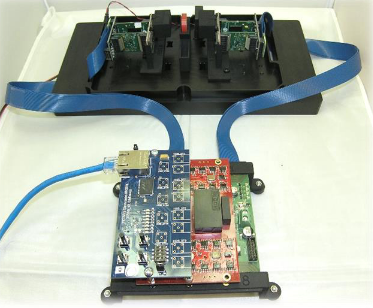
\includegraphics[scale=0.6]{3DesignPrinciples/32Tritium_detector/PETSYS_System.png}
\caption{Different parts of PETSYS system.\label{fig:PETSYS}~\cite{PETSYS}}
\end{figure}

Taking into account the current detection limits imposed, this capacity should be enough for TRITIUM detector but, as we will see in chapter \ref{chap:Prototypes}, TRITIUM is a modular detector. If we need to overcome its limits reached (improve its sensitivity or reduce their background even more) we will need to increase this capacity. We need an electronic system that is able to increase its capacity in a modular way and PETSYS meets this requirement. It has the Clock and Trigger module with which we have the possibility of connecting up to sixteen different PETSYS basic boards in parallel with which we could read up to 16384 SiPM\footnote{$1024\cdot{}16 = 16384$}.

PETSYS is based on C++ and Python scripts that are prepared for the main tasks required for our experiment, such as time coincidence options between SiPM (or even SiPM matrices) or energy discrimination. In addition, PETSYS is open source, so if it is necessary, we have the option to modify the scripts for developing interesting functions. The way the signals will be processed and analyzed for PETSYS will be exactly the same as those shown in Figure \ref{fig:ElectronicConfiguraitonsPMT}

This system has a time resolution of $250~\pico\second$ which is one of the best time resolutions of commercial systems available today and its price is around $10$\euro$/$ channel, which is very cheap in comparison with current similar electronic systems.

As we will see in section \ref{sec:CharacterizationSiPM}, the temperature of each SiPM matrix is an important parameter to take into account. The PETSYS system has the ability to monitor the temperature of both, the SiPM matrices and ASICS that are used to control them during the measurements.

Although PETSYS is the system used to work with SiPM matrices in the TRITIUM detector, it does not allow characterizing the SiPMs, which is an important task to understand the results of our detector.

In order to do so, we have designed, developed and built an electronic system with which we can read up to eight different SiPMs. With this system we can also monitor the temperature of the SiPMs used.

This system is based on three different PCBs\footnote{PCB, Printed Circuit Board}, which are shown in Figure \ref{fig:PCBs_LEDSpectrum} and whose electronical schemes are shown in the appendix \ref{App:ElectronicalSchemesSiPMPCBs}:

\begin{enumerate}
\item{} The first PCB, shown in Figure \ref{subfig:PCB1}, is used to organize the SiPMs and sensor temperature in this system. This PCB has the ability to place up to 8 different SiPMs and a temperature sensor and arrange these signals on two HDMI connections.

This PCB will be inside a special black box, from "" company, that has a high degree of light tightness. This black box has a small hole, whose diameter is $1~\mm$, prepared to introduce an optical fiber\footnote{The optical fiber used is BCF-98 from Saint-Gobain company \cite{OpticalFibers}} with which we will illuminate the SiPM with a incoherent light source. The light source used is a LED, model 430L from Thorlabs company \cite{LEDThorlabs}, whose emission spectrum is shown in Figure \ref{subfig:LEDSpectrum}, which has been experimentaly measured using a spectrometer and fitted to a Gaussian function. We can see that the emission peak of this LED is produced at $436.3$ with a FWHM\footnote{The FWHM parameter, Full Width at Half Maximum, of a Gaussian fit can be calculated from its sigma using the equation: FWHM$=2.35 \cdot{} \sigma$} of $19.1~\nano\meter$. With this LED we intend to simulate the light emission of the fibers used in the TRITIUM experiment to calibrate the SiPMs at the working wavelength. 

\item{} The second PCB, shown in Figure \ref{subfig:PCB2}, is used to sum the different signals from the SiPMs used in the first PCB and amplify the output signal by a factor G. This PCB uses a differential amplification with which we achieve to reduce the electronic noise of the system.

\item{} The third PCB, shown in Figure \ref{subfig:PCB3}, is used to arrange all the different input and output signals of this system in an HDMI connection with which we connect to the second PCB. The objective of this PCB is to avoid the introduction of electrical noise by crosstalk between different signals.

The input signals of this system are the supply voltage of the SiPMs and the supply voltage of the PCBs ($\pm 6~\volt$) and the output signals of this system are the temperature sensor signal and the summed signal of all SiPMs. 

\end{enumerate}

\begin{figure}[htbp]
 \centering
  \subfloat[PCB 1 used to arrang 8 SiPMs and black box.]{
   \label{subfig:PCB1}
    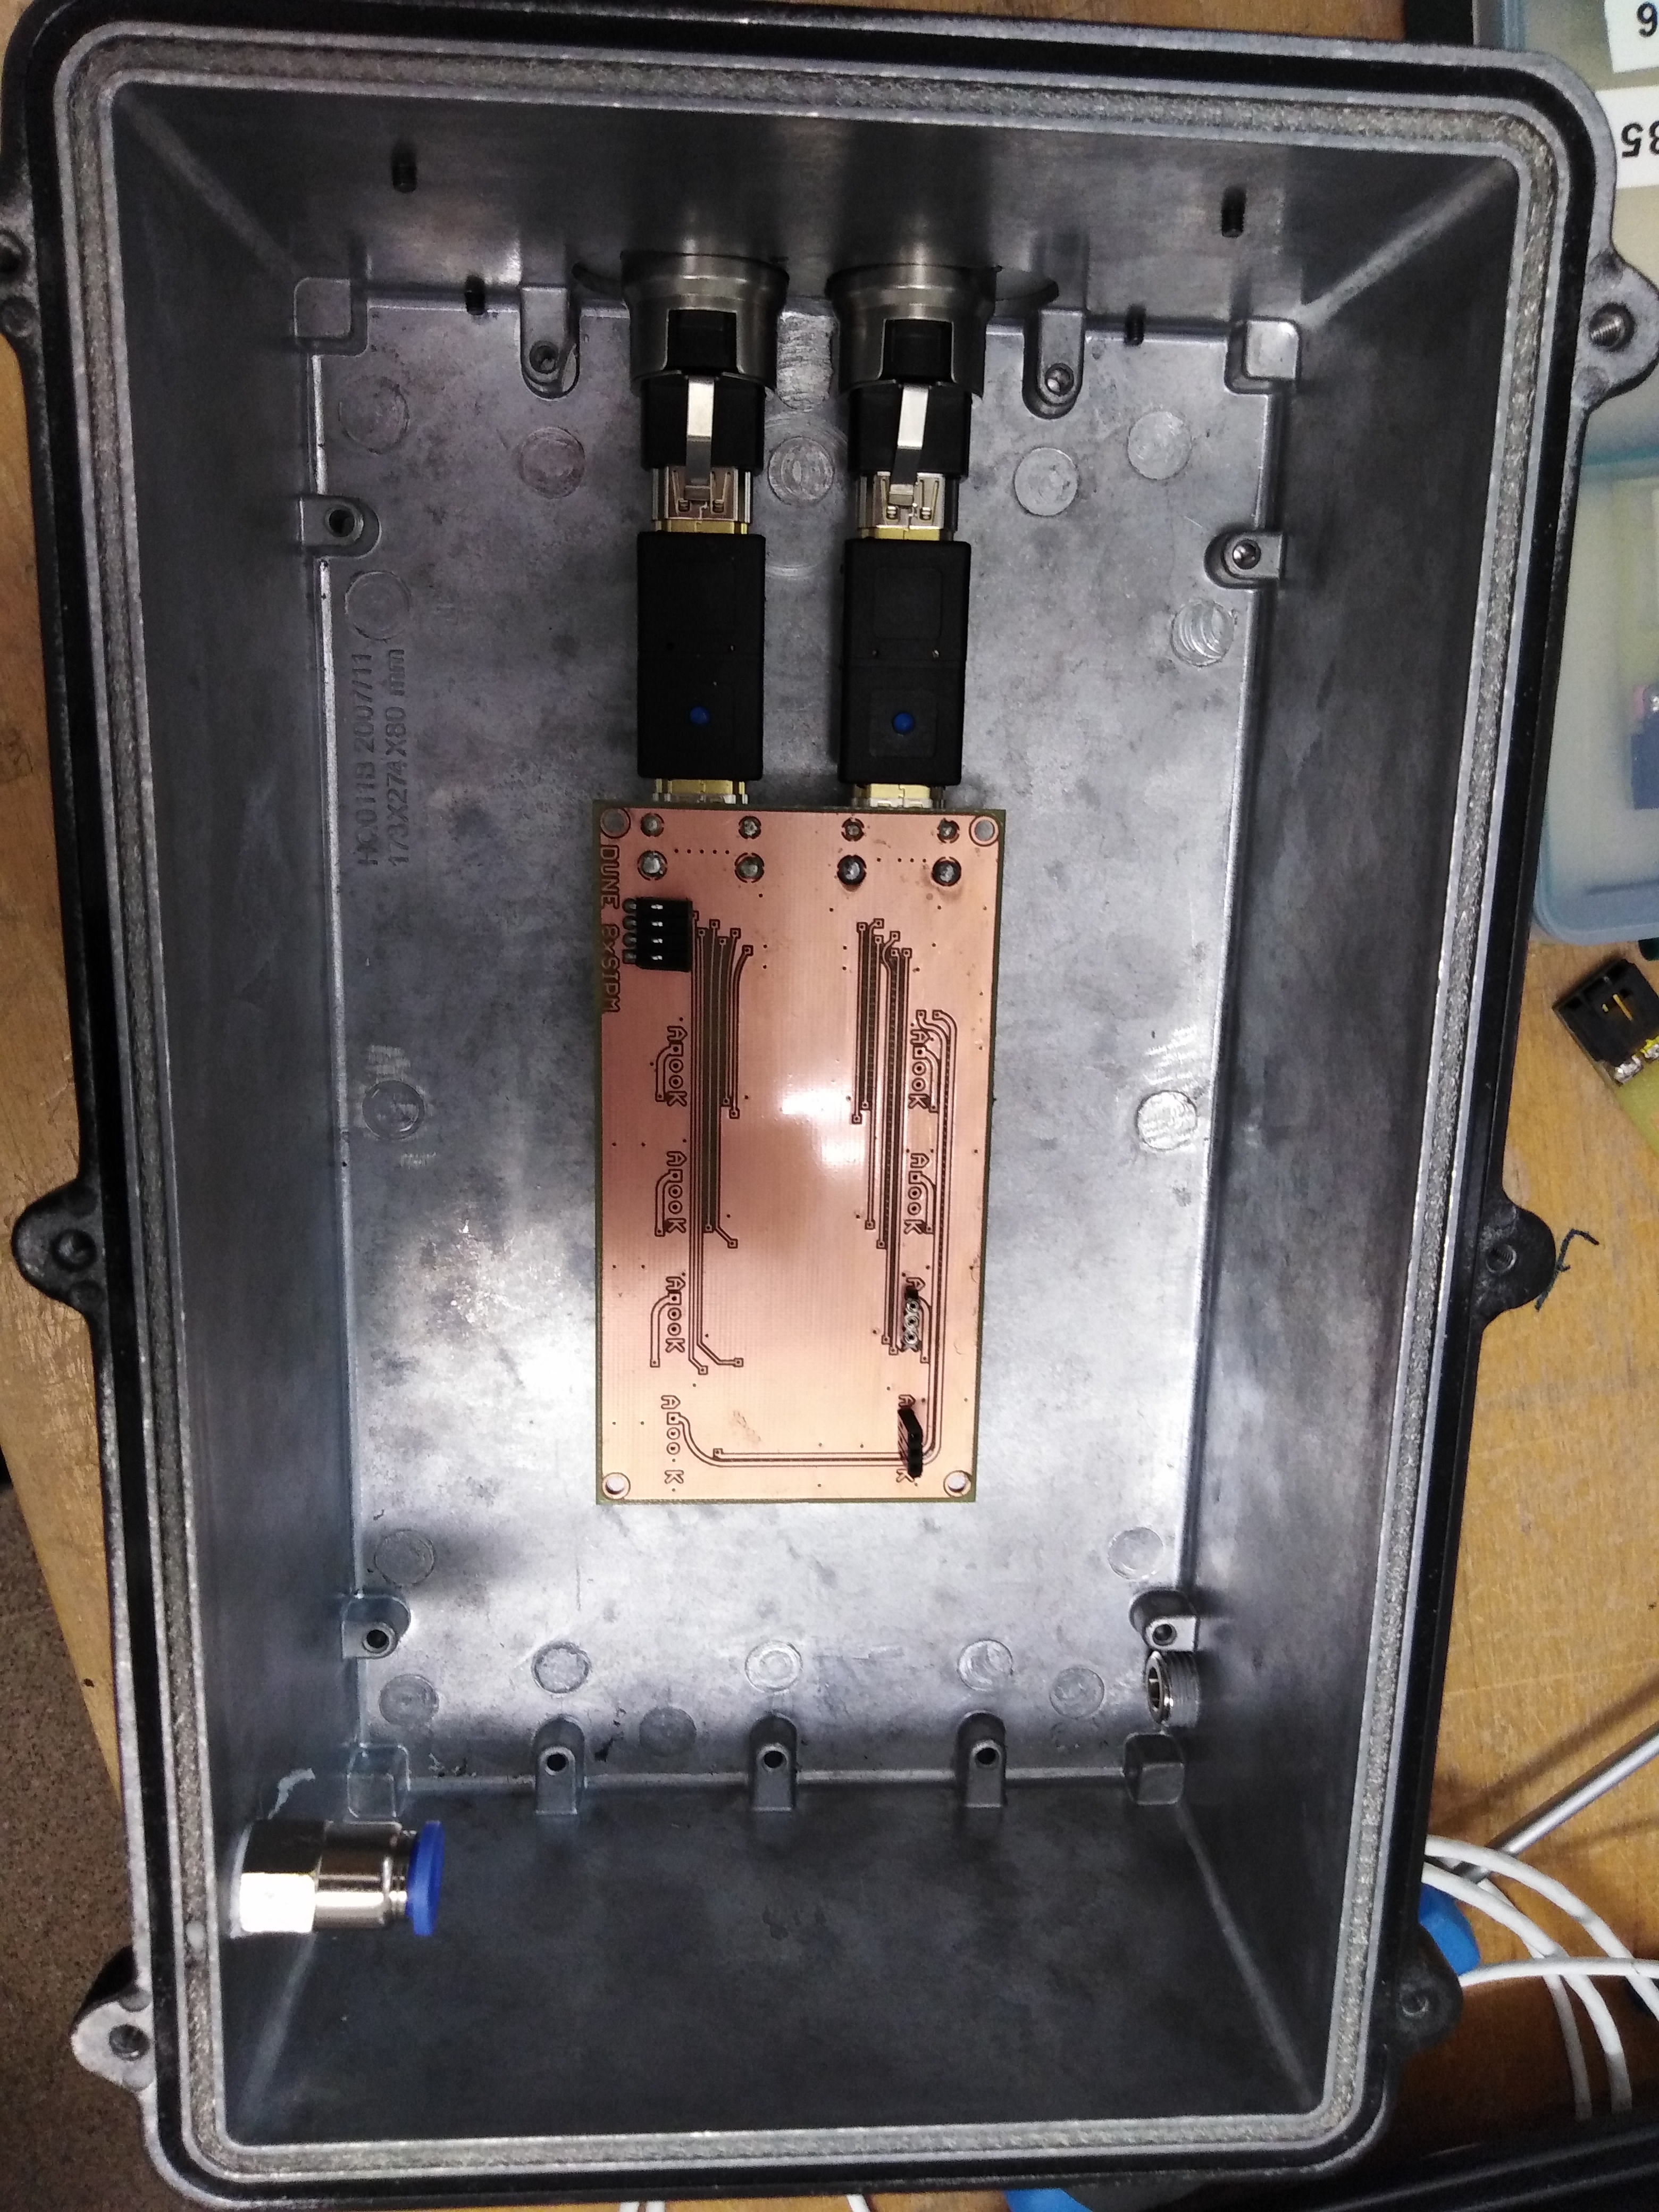
\includegraphics[angle=90,width=0.5\textwidth]{3DesignPrinciples/32Tritium_detector/PCB1_SiPM_Black_Box.jpg}}
  \subfloat[PCB 2 used to sum and amplify the output signals of SiPMs]{
   \label{subfig:PCB2}
    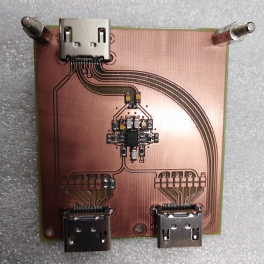
\includegraphics[width=0.45\textwidth]{3DesignPrinciples/32Tritium_detector/PCB2_SIPMs.png}}
   \newline
  \subfloat[PCB 3 used to arrange the different singals of the system.]{
   \label{subfig:PCB3}
    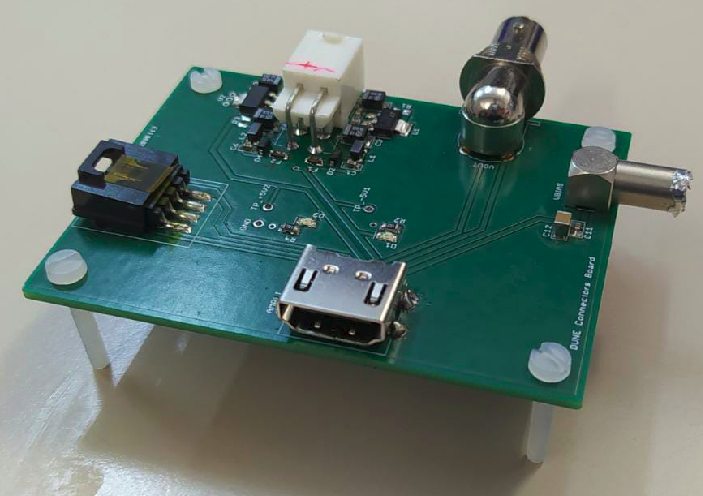
\includegraphics[width=0.4\textwidth]{3DesignPrinciples/32Tritium_detector/PCB3_SiPMs.png}}
    \subfloat[Emission spectrum of the LED.]{
   \label{subfig:LEDSpectrum}
    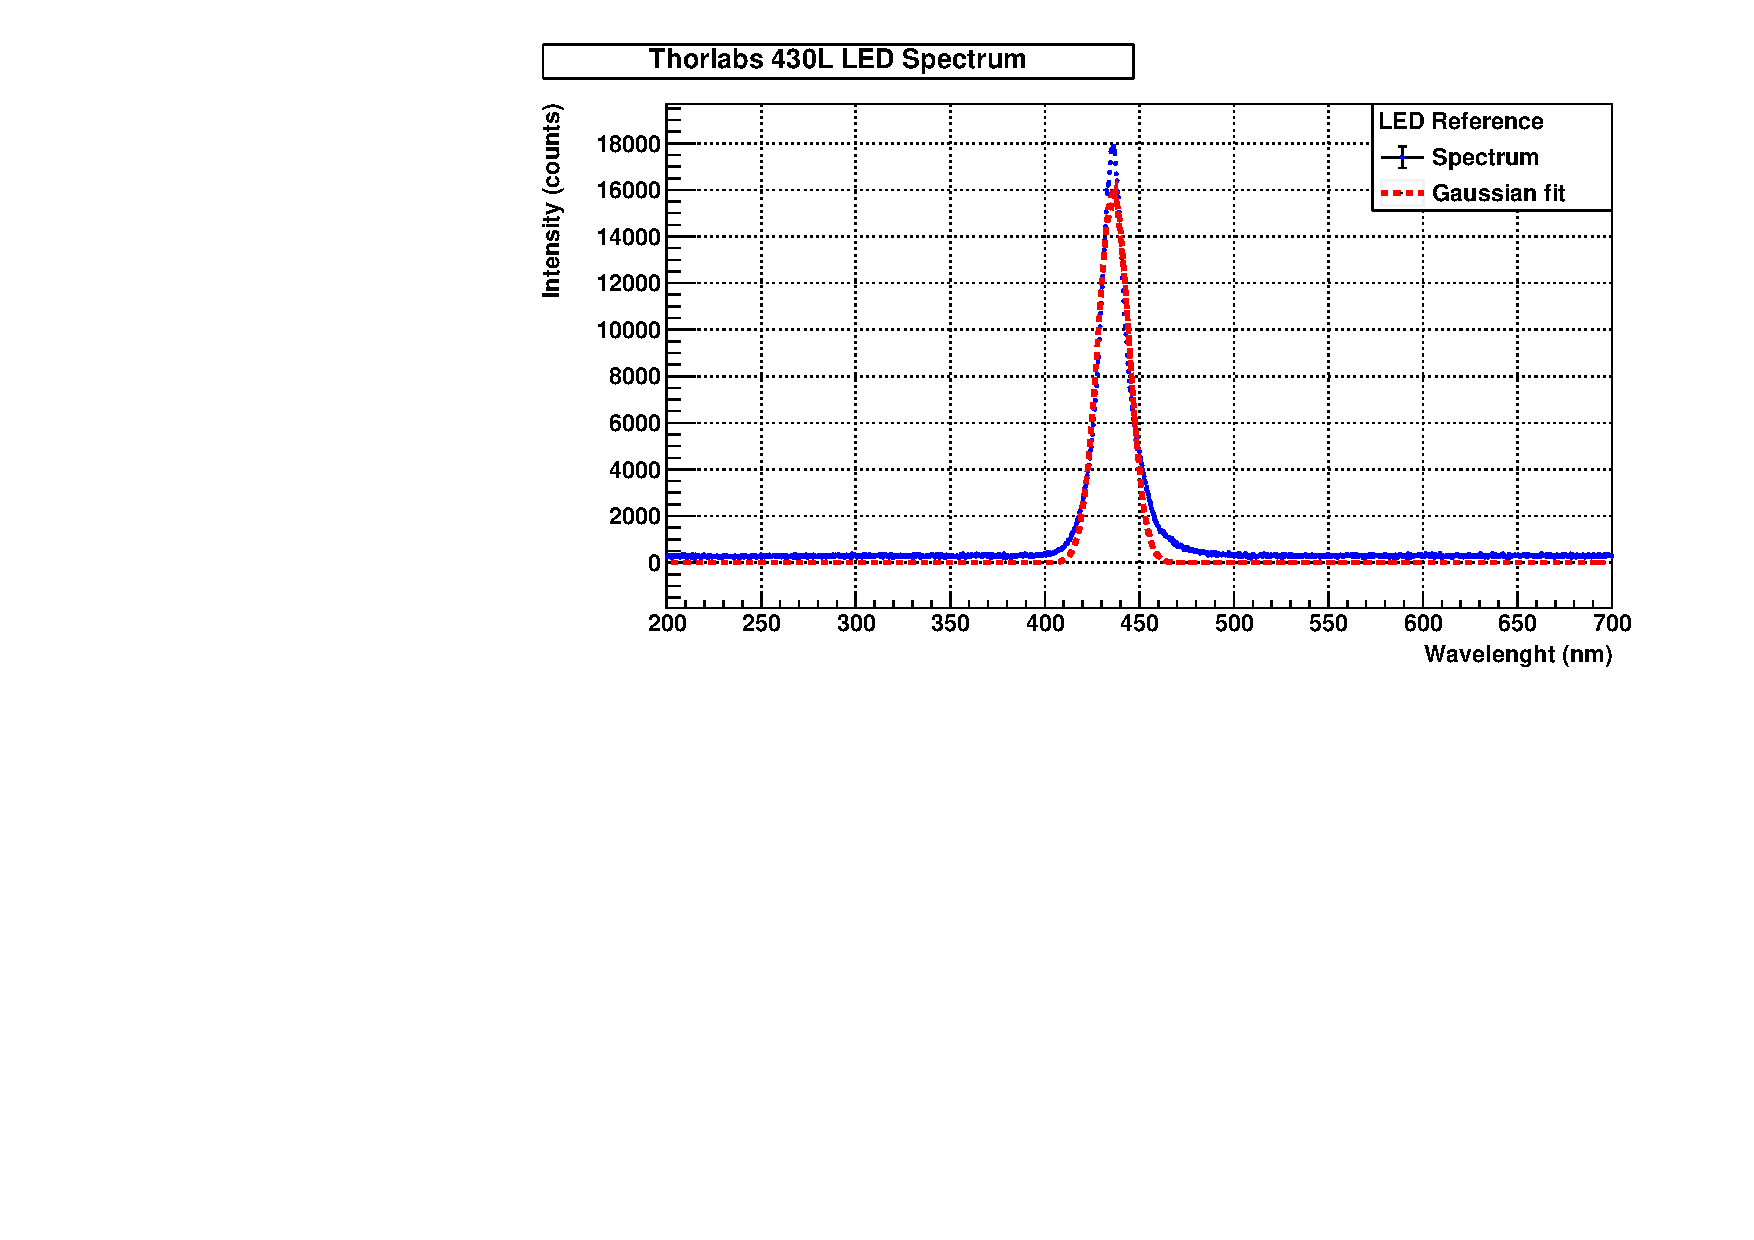
\includegraphics[width=0.6\textwidth]{3DesignPrinciples/32Tritium_detector/LED_DUNE.pdf}}
 \caption{Three PCBs used for the SiPM characterization and LED emission spectrum.}
 \label{fig:PCBs_LEDSpectrum}
\end{figure}